\documentclass[10pt,twocolumn]{article}

% Minimal packages for fast compile
\usepackage{times}
\usepackage[utf8]{inputenc}
\usepackage[T1]{fontenc}
\usepackage[a4paper,margin=2cm]{geometry}
\usepackage{titlesec}
\usepackage{graphicx}
\usepackage{booktabs}
\usepackage{float}
\usepackage[section]{placeins}

% Section title styles (as in your reference)
\titleformat{\section}{\bfseries\fontsize{12}{14}\selectfont}{\thesection.}{0.5em}{}
\titleformat{\subsection}{\bfseries\fontsize{11}{13}\selectfont}{\thesubsection.}{0.5em}{}

\title{\textbf{Project Plan }}
\author{Chinmay Purandare\\
Lorenzo Parata\\
Chongnan Wang\\
Xiaotian Jiang \\
Xinxin Qin \\
Department of Electronics\\
KTH Royal Institute of Technology\\
Stockholm, Sweden\\
Emails: chinmayp@kth.se, parata@ug.kth.se, chongnan@kth.se, xjia@kth.se, xinxinq@kth.se}
\date{}

\begin{document}
\maketitle


\section{Background}
This project continues previous work at KTH developing digital electronics for extreme high-temperature environments, specifically targeting Venus surface conditions. Last year's students successfully designed and synthesized two RISC-V processor variants—a parallel model in VHDL and a bit-serial CISC-V model in ProGram—both optimized for the 12-pad constraint of KTH's high-temperature test station. However, they did not complete FPGA implementation and testing.\\
The current project addresses this gap by implementing and testing both processor models on FPGAs, developing an advanced testbench on a separate FPGA, and integrating the multi-FPGA system to validate functionality. This work uses KTH's experimental Silicon-on-Insulator technology, which can operate at temperatures approaching Venus's 480°C requirement, and leverages the open-source RISC-V architecture to avoid licensing constraints.\\
The project requires expertise in hardware design, software development, FPGA implementation, and system integration, with support from supervisors Artur Podobas (RISC-V/compiler) and Johnny Öberg (ProGram/FPGA). Success will validate these designs for eventual ASIC fabrication and demonstrate processor viability for extreme-environment applications.


\section{Organization}
The primary objective of this project is to design, implement, and rigorously validate two distinct processor architectures—a standard RISC-V core and a novel Bit-Serial CISC-V core—by developing a robust, dual-FPGA prototyping and validation system. This will be achieved within a structured 4-month timeline, ensuring all outcomes are specific, measurable, and demonstrable.\\
To validate these designs beyond software simulation, we will create an advanced testbench system deployed on a second, separate FPGA. This testbench will incorporate synthesized program memory, a UART controller for PC communication, and a GPIO controller to emulate peripherals. The processor-under-test on one FPGA and the testbench on the other will be physically interconnected via a defined GPIO/PMOD interface to form a complete, operational computer system.\\
Success will be quantitatively measured through a phased verification process. First, both cores must successfully output a "Hello World" message via UART. Second, they must achieve a 100\% pass rate on a comprehensive suite of at least 10 assembly-level test programs covering core ISA functionality. Finally, both must correctly execute a complex benchmark algorithm (e.g., CoreMark or matrix multiplication), with results transmitted back to the host PC for verification. System integration will be deemed successful upon stable data transfer of over 1,000 instructions without corruption. Furthermore, we will collect and report key performance metrics, including maximum clock frequency (Fmax), execution cycle counts for benchmarks, and FPGA resource utilization (LUTs, FFs, BRAM) for a direct architectural comparison.\\
This goal is achievable as it leverages mature tools (FPGA design suites, RISC-V toolchains) and a phased development approach, mitigating risk by initially verifying cores in simulation and on a single FPGA before final dual-FPGA integration. The project is highly relevant as it provides a critical, empirical validation of the novel Bit-Serial CISC-V architecture against the established RISC-V standard, creating a foundational platform for future architectural research and development. The entire project, from RTL design to final system verification and performance analysis, will be completed within the 16-week timeframe.


\section{Description of how we are working}
Our group has chosen to follow an agile approach to manage the project. We took that decision to remain flexible and adapt as quickly as possible in case of new findings or challenges during development. Indeed, in our case there is not one way to complete the final objective and it can be interesting to have the possibility to change path at some point.\\
We will work in weekly sprints. Indeed, every Monday, we will hold a meeting to plan the upcoming sprint. During this meeting, we will define our sprint goals, assign specific tasks to each team member, and estimate the expected outcomes.\\
We may also hold another sprint Review at every sprint. We will review the progress, demonstrate what has been achieved, point at difficulties and find solutions together. A short retrospective will also be held to discuss what went well, what could be improved, and how to adjust our workflow for the next sprint.\\
The project is divided into three main parts:

\begin{itemize}
  \item \textbf{RISC-V processor} — focusing on the bit-parallel implementation.
  \item \textbf{CISC-V (bit-serial RISC-V)} — focusing on the serial version and its specific constraints.
  \item \textbf{Testbench (TB)} — focusing on a functional and scalable test environment to verify both processor versions.
\end{itemize}
Each subgroup will be responsible for its own sprint but will coordinate closely with the others to ensure compatibility at the end.


\section{Communicate with each other and other stakeholders}
Effective communication is essential for coordinating our work and ensuring smooth progress throughout the project. We use several communication channels, each with a specific purpose.We are using Whatsapp for everyday communication within the group. It allows quick discussions, sharing short updates, and coordinating meetings or deadlines.We are also using Discord for online meetings, screen sharing, and document discussions. It provides a more organized environment for technical conversations and group reviews compared to instant messaging.
But our central collaboration platform is GitHub for both code development and documentation. We also use the repository to collaborate on written assignments, using LaTeX, such as this one.Finally we are using mail and zoom meetings for formal communication with supervisors and professors, including submitting deliverables, asking for clarifications, or discussing project milestones.This combination of tools ensures that our communication remains efficient, clear and traceable.

\FloatBarrier
\section{Work Breakdown Structure (WBS)}
\begin{figure}[t]
\centering
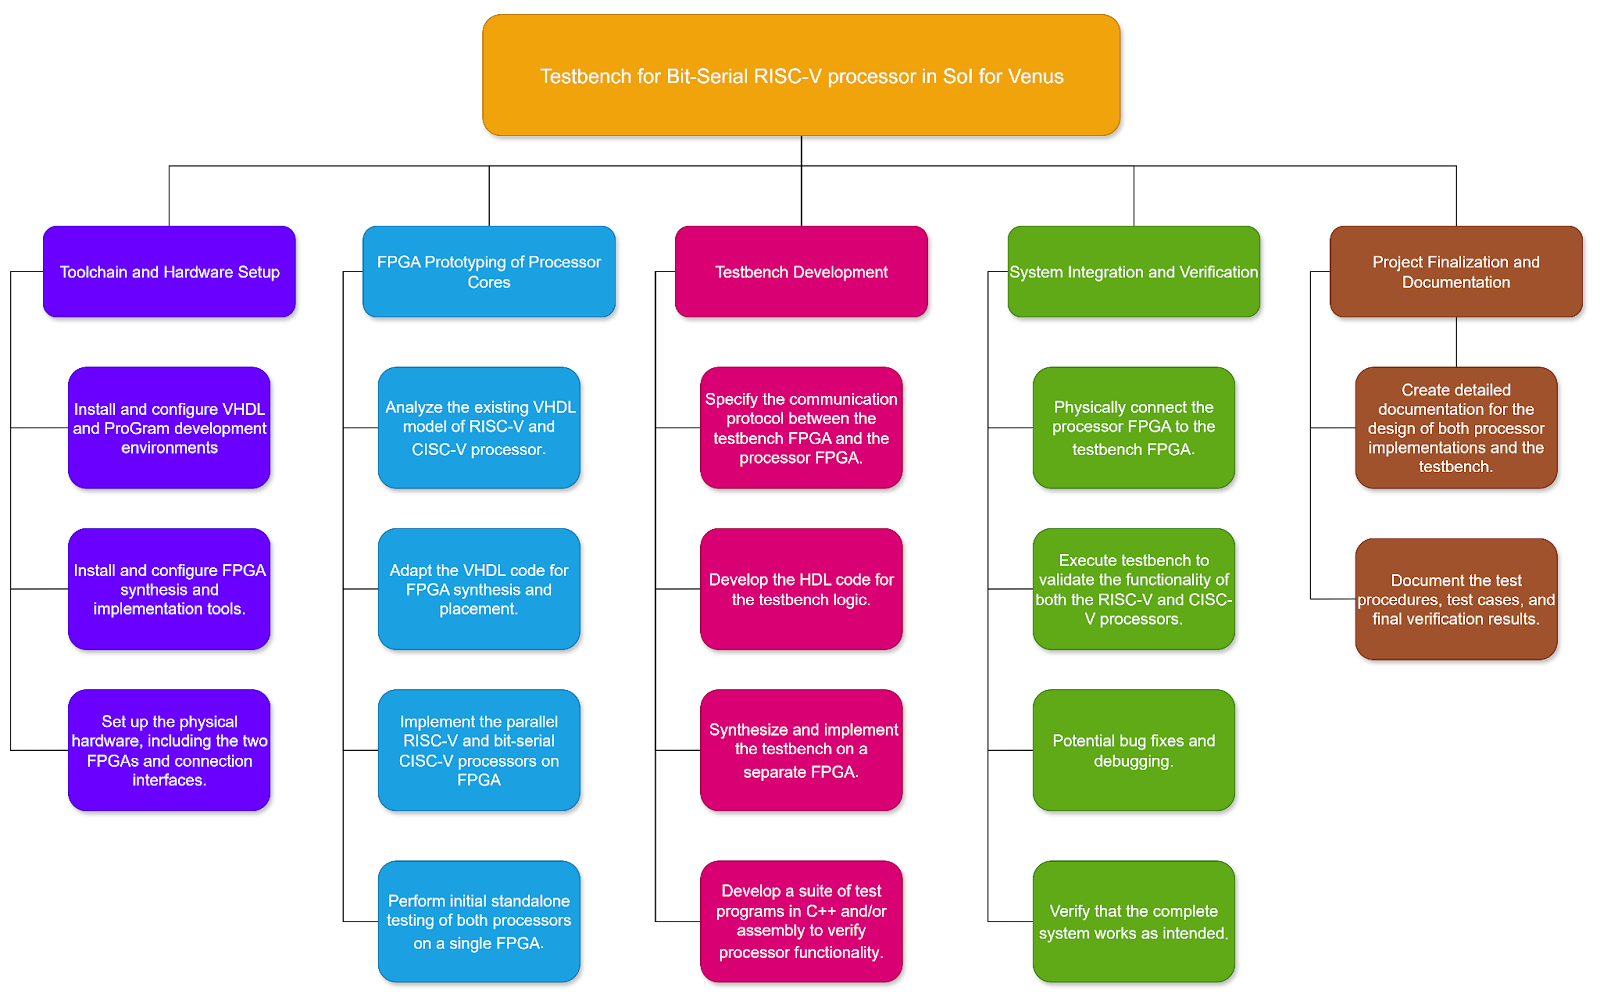
\includegraphics[width=\linewidth]{WBS.png}
\caption{Work Breakdown Structure (WBS)}
\label{fig:timeline}
\end{figure}

\section{Global plan}
\subsection{}
\section{First sprint plan}



\end{document}
